\documentclass[a4paper, 14pt]{extarticle}

% Поля
%--------------------------------------
\usepackage{geometry}
\geometry{a4paper,tmargin=2cm,bmargin=2cm,lmargin=3cm,rmargin=1cm}
%--------------------------------------


%Russian-specific packages
%--------------------------------------
\usepackage[T2A]{fontenc}
\usepackage[utf8]{inputenc} 
\usepackage[english, main=russian]{babel}
%--------------------------------------

\usepackage{textcomp}

% Красная строка
%--------------------------------------
\usepackage{indentfirst}               
%--------------------------------------             


%Graphics
%--------------------------------------
\usepackage{graphicx}
\graphicspath{ {../images/} }
\usepackage{wrapfig}
%--------------------------------------

% Полуторный интервал
%--------------------------------------
\linespread{1.3}                    
%--------------------------------------

%Выравнивание и переносы
%--------------------------------------
% Избавляемся от переполнений
\sloppy
% Запрещаем разрыв страницы после первой строки абзаца
\clubpenalty=10000
% Запрещаем разрыв страницы после последней строки абзаца
\widowpenalty=10000
%--------------------------------------

%Списки
\usepackage{enumitem}

%Подписи
\usepackage{caption} 

%Гиперссылки
\usepackage{hyperref}

\hypersetup {
	unicode=true
}

%Рисунки
%--------------------------------------
\DeclareCaptionLabelSeparator*{emdash}{~--- }
\captionsetup[figure]{labelsep=emdash,font=onehalfspacing,position=bottom}
%--------------------------------------

% \usepackage{tempora}

%Листинги
%--------------------------------------
\usepackage{listings}
\lstset{
  basicstyle=\ttfamily\footnotesize, 
  %basicstyle=\footnotesize\AnkaCoder,        % the size of the fonts that are used for the code
  breakatwhitespace=false,         % sets if automatic breaks shoulbd only happen at whitespace
  breaklines=true,                 % sets automatic line breaking
  captionpos=t,                    % sets the caption-position to bottom
  inputencoding=utf8,
  frame=single,                    % adds a frame around the code
  keepspaces=true,                 % keeps spaces in text, useful for keeping indentation of code (possibly needs columns=flexible)
  keywordstyle=\bf,       % keyword style
  numbers=left,                    % where to put the line-numbers; possible values are (none, left, right)
  numbersep=5pt,                   % how far the line-numbers are from the code
  xleftmargin=25pt,
  xrightmargin=25pt,
  showspaces=false,                % show spaces everywhere adding particular underscores; it overrides 'showstringspaces'
  showstringspaces=false,          % underline spaces within strings only
  showtabs=false,                  % show tabs within strings adding particular underscores
  stepnumber=1,                    % the step between two line-numbers. If it's 1, each line will be numbered
  tabsize=2,                       % sets default tabsize to 8 spaces
  title=\lstname                   % show the filename of files included with \lstinputlisting; also try caption instead of title
}
%--------------------------------------

%%% Математические пакеты %%%
%--------------------------------------
\usepackage{amsthm,amsfonts,amsmath,amssymb,amscd}  % Математические дополнения от AMS
\usepackage{mathtools}                              % Добавляет окружение multlined
\usepackage[perpage]{footmisc}
%--------------------------------------

%--------------------------------------
%			НАЧАЛО ДОКУМЕНТА
%--------------------------------------

\begin{document}

%--------------------------------------
%			ТИТУЛЬНЫЙ ЛИСТ
%--------------------------------------
\begin{titlepage}
    \thispagestyle{empty}
    \newpage


    %Шапка титульного листа
    %--------------------------------------
    \vspace*{-60pt}
    \hspace{-65pt}
    \begin{minipage}{0.3\textwidth}
        \hspace*{-20pt}\centering
        \includegraphics[width=\textwidth]{emblem}
    \end{minipage}
    \begin{minipage}{0.67\textwidth}\small \textbf{
            \vspace*{-0.7ex}
            \hspace*{-6pt}\centerline{Министерство науки и высшего образования Российской Федерации}
            \vspace*{-0.7ex}
            \centerline{Федеральное государственное бюджетное образовательное учреждение }
            \vspace*{-0.7ex}
            \centerline{высшего образования}
            \vspace*{-0.7ex}
            \centerline{<<Московский государственный технический университет}
            \vspace*{-0.7ex}
            \centerline{имени Н.Э. Баумана}
            \vspace*{-0.7ex}
            \centerline{(национальный исследовательский университет)>>}
            \vspace*{-0.7ex}
            \centerline{(МГТУ им. Н.Э. Баумана)}}
    \end{minipage}
    %--------------------------------------

    %Полосы
    %--------------------------------------
    \vspace{-25pt}
    \hspace{-35pt}\rule{\textwidth}{2.3pt}

    \vspace*{-20.3pt}
    \hspace{-35pt}\rule{\textwidth}{0.4pt}
    %--------------------------------------

    \vspace{1.5ex}
    \hspace{-35pt} \noindent \small ФАКУЛЬТЕТ\hspace{80pt} <<Информатика и системы управления>>

    \vspace*{-16pt}
    \hspace{47pt}\rule{0.83\textwidth}{0.4pt}

    \vspace{0.5ex}
    \hspace{-35pt} \noindent \small КАФЕДРА\hspace{50pt} <<Теоретическая информатика и компьютерные технологии>>

    \vspace*{-16pt}
    \hspace{30pt}\rule{0.866\textwidth}{0.4pt}

    \vspace{11em}

    \begin{center}
        \Large {\bf Лабораторная работа №2а} \\
        \large {\bf по курсу <<Языки и методы программирования>>} \\
        \large <<Модель вселенной>>
    \end{center}\normalsize

    \vspace{8em}


    \begin{flushright}
        {Студент группы ИУ9-22Б Бойко Р. А. \hspace*{15pt}\\
            \vspace{2ex}
            Преподаватель Посевин Д. П.\hspace*{15pt}}
    \end{flushright}

    \bigskip

    \vfill


    \begin{center}
        \textsl{Москва 2024}
    \end{center}
\end{titlepage}
%--------------------------------------
%		КОНЕЦ ТИТУЛЬНОГО ЛИСТА
%--------------------------------------

\renewcommand{\ttdefault}{pcr}

\setlength{\tabcolsep}{3pt}
\newpage
\setcounter{page}{2}

\section{Задание}\label{Sect::task}

Реализовать модель вселенной. Каждый элемент вселенной должен быть объектом
некоего публичного класса, который инициализируется вспомогательным публичным
классом порождающим эту вселенную. При инициализации экземпляров класса частиц
моделируемой вселенной необходимо подсчитывать количество частиц вселенной используя
статичное экземплярное поле защищенное от изменения из объектов внешних классов путем
реализации статичного метода. Сформировать исходные данные и определить необходимые
экземплярные поля для хранения состояния объектов частиц вселенной в соответствии с
условием задачи и реализовать расчет.
Вычислить силу притяжения действующую на произвольную частицу массой M, 
находящейся в заданной координате пространства со стороны всех частиц вселенной.

\section{Результаты}\label{Sect::res}

Исходный код программы представлен в листингах~\ref{lst:code1}--~\ref{lst:code3}.

\begin{lstlisting}[language={},caption={класс Particle},label={lst:code1}]
public class Particle {
    private double mass;
    private double x;
    private double y;
    private double z;

    public Particle(double mass, double x, double y, double z) {
        this.mass = mass;
        this.x = x;
        this.y = y;
        this.z = z;
    }

    public double getMass() {
        return mass;
    }

    public double getX() {
        return x;
    }

    public double getY() {
        return y;
    }

    public double getZ() {
        return z;
    }
}    
\end{lstlisting}

\begin{lstlisting}[language={},caption={класс Universe},label={lst:code2}]
public class Universe {
    private static final int MAX_PARTICLES = 1000; // Максимальное количество частиц
    private static Particle[] particles = new Particle[MAX_PARTICLES];
    private static int totalParticles = 0; // Текущее количество частиц во вселенной
    public static final double GRAVITATIONAL_CONSTANT = 6.67430e-11; // Гравитационная постоянная

    public static void addParticle(Particle particle) {
        if (totalParticles < MAX_PARTICLES) {
            particles[totalParticles++] = particle;
        } else {
            System.out.println("Cannot add more particles. Universe is full.");
        }
    }

    public static int getTotalParticles() {
        return totalParticles;
    }

    public static double getVectorLength(double x, double y, double z) {
        return Math.sqrt(Math.pow(x, 2) + Math.pow(y, 2) + Math.pow(z, 2));
    }

    public static double getForceMagnitude(double m1, double m2, double r) {
        return (GRAVITATIONAL_CONSTANT * m1 * m2) / Math.pow(r, 2);

    }

    public static double calculateAttractionForce(Particle particle) {
        double totalForceX = 0.0;
        double totalForceY = 0.0;
        double totalForceZ = 0.0;
        for (int i = 0; i < totalParticles; i++) {
            Particle universeParticle = particles[i];
            if (!particle.equals(universeParticle)) {
                double deltaX = universeParticle.getX() - particle.getX();
                double deltaY = universeParticle.getY() - particle.getY();
                double deltaZ = universeParticle.getZ() - particle.getZ();
                double distance = getVectorLength(deltaX, deltaY, deltaZ);
                double forceMagnitude = getForceMagnitude(particle.getMass(), universeParticle.getMass(), distance);
                totalForceX += forceMagnitude * (deltaX / distance);
                totalForceY += forceMagnitude * (deltaY / distance);
                totalForceZ += forceMagnitude * (deltaZ / distance);
            }
        }
        return getVectorLength(totalForceX, totalForceY, totalForceZ);
    }
}
\end{lstlisting}

\begin{lstlisting}[language={},caption={класс Test},label={lst:code3}]
public class Test {
    public static void main(String[] args) {
        Universe.addParticle(new Particle(10, 0, 0, 0));
        Universe.addParticle(new Particle(5, 1, 1, 1));
        Universe.addParticle(new Particle(8, -1, -1, -1));
        Universe.addParticle(new Particle(20, -5, 0, 3));
        Universe.addParticle(new Particle(15, -8, 45, 3));
        Universe.addParticle(new Particle(55, 3, 1, 8));
        Universe.addParticle(new Particle(28, -5, 7, -15));
        Universe.addParticle(new Particle(30, -7, 10, 36));
        System.out.println("Total particles in the universe: " + Universe.getTotalParticles());
        System.out.println(Universe.calculateAttractionForce(new Particle(35, 6, 5, 2)));
    }
}    
\end{lstlisting}

Результат запуска представлен на рисунке~\ref{fig:lab2a}.

\begin{figure}[!htb]
    \centering
    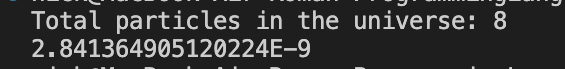
\includegraphics[width=0.8\textwidth]{lab2a}
    \caption{Результат}
    \label{fig:lab2a}
\end{figure}

\end{document}
